% !TeX program = xelatex
% !TeX encoding = UTF-8

%% --------------------------------------------------------------------------------
%% Tongji-Beamer Example Document
%%
%% Tongji-Beamer 是基于 SJTUBeamer (https://github.com/sjtug/SJTUBeamer) 改造的
%% 同济大学风格 Beamer 主题。视觉素材来自 TJ-CSCCG/tongji-visual 项目。
%%
%% 在此致谢 SJTUBeamer 原作者 (CC-BY-NC-SA 4.0) 与 tongji-visual 维护者。
%%
%% --------------------------------------------------------------------------------
%% 关于分文件：
%%   本 demo 把所有特性放在单一 main.tex 是为了让 fork 模板的人一眼看全功能。
%%   实际写答辩/汇报时建议改成：
%%
%%   \begin{document}
%%     \input{sections/cover.tex}
%%     \input{sections/01-intro.tex}     % §1 引言
%%     \input{sections/02-method.tex}    % §2 方法
%%     \input{sections/03-results.tex}   % §3 实验
%%     \input{sections/04-conclusion.tex}% §4 总结
%%     \input{sections/thanks.tex}
%%   \end{document}
%%
%%   每个 section 文件里只写自己的 \section{...} + frames。
%% --------------------------------------------------------------------------------

% fontset=none 关闭 ctex 默认字体集，下面手动指定 Noto CJK 以获得更好观感
\documentclass[xcolor=table,dvipsnames,svgnames,aspectratio=169,fontset=none]{ctexbeamer}

\usepackage{tikz}
\usepackage[normalem]{ulem}
\usetikzlibrary{arrows,positioning,shadows.blur}
\usepackage{amsmath}
\usepackage{graphicx}
\usepackage{hologo}
\usepackage{colortbl}
\usepackage{booktabs}
\usepackage{listings}
\usepackage{datetime2}
\usepackage{fontawesome5}
\usepackage{hyperref}
\usepackage{eso-pic}

% ============== 字体 ==============
% 设计：标题用 Noto Sans CJK SC（黑体，醒目），正文用 Noto Serif CJK SC（宋体，易读）
\setCJKmainfont{Noto Serif CJK SC}[BoldFont={Noto Serif CJK SC Bold}]
\setCJKsansfont{Noto Sans CJK SC}[BoldFont={Noto Sans CJK SC Bold}]
\setCJKmonofont{Noto Sans Mono CJK SC}
\setCJKfamilyfont{kai}{LXGW WenKai}
\setCJKfamilyfont{songti}{Noto Serif CJK SC}[BoldFont={Noto Serif CJK SC Bold}]
\setCJKfamilyfont{heiti}{Noto Sans CJK SC}[BoldFont={Noto Sans CJK SC Bold}]
\newcommand{\kaiti}{\CJKfamily{kai}}
\newcommand{\songti}{\CJKfamily{songti}}
\newcommand{\heiti}{\CJKfamily{heiti}}

% Beamer 正文用 serif（CJK 默认 \rmfamily = Noto Serif CJK SC）
\usefonttheme{serif}
% 标题、frametitle、section、blocks 仍用 sans 黑体
\setbeamerfont{title}{family=\sffamily,series=\bfseries}
\setbeamerfont{subtitle}{family=\sffamily}
\setbeamerfont{frametitle}{family=\sffamily,series=\bfseries}
\setbeamerfont{section in head/foot}{family=\sffamily}
\setbeamerfont{section in toc}{family=\sffamily,series=\bfseries}
\setbeamerfont{block title}{family=\sffamily,series=\bfseries}
\setbeamerfont{author}{family=\sffamily}
\setbeamerfont{institute}{family=\sffamily}
\setbeamerfont{date}{family=\sffamily}

\hypersetup{
  unicode            = true,
  pdfdisplaydoctitle = true
}

\renewcommand{\TeX}{\hologo{TeX}}
\renewcommand{\LaTeX}{\hologo{LaTeX}}
\newcommand{\XeLaTeX}{\hologo{Xe}\kern-.13em\LaTeX{}}
\newcommand{\beamer}{\textsc{beamer}}
\newcommand{\TongjiBeamer}{\textsc{Tongji-Beamer}}

\usetheme[max,blue,light]{tjbeamer}
% 使用 maxplus/max/min 切换标题页样式
% 使用 red/blue 切换主色调（blue=同济蓝，red=同济红+金）
% 使用 light/dark 切换亮/暗模式

% color theme 把 background canvas 设为 bg=white（默认模板会铺满白色），会盖掉 shipout BG
% 显式清空 canvas 模板，让 \AddToShipoutPictureBG 的图层可见
\setbeamertemplate{background canvas}{}
\setbeamertemplate{background}{}

% frametitle 默认 bg=white 会形成大白块挡住背景；改成透明
\setbeamercolor{frametitle}{bg=,fg=cprimary}

% Beamer 默认导航按钮太多（slide/frame/subsection/section/doc/back-find-forward 七组），
% 只保留常用：单张幻灯片上一/下一 + 历史返回/前进 + 页码 N/总数
\setbeamertemplate{navigation symbols}{%
  \insertslidenavigationsymbol%
  \insertbackfindforwardnavigationsymbol%
  \hspace*{0.5em}%
  {\usebeamerfont{footline}\color{black!50}\insertframenumber/\inserttotalframenumber}%
  \hspace*{0.3em}%
}

% 隐藏右下角小校徽（主题自带的 logo template）
\setbeamertemplate{logo}{}

% miniframes 主题的页顶分隔色条（在 section 导航条下方），不需要时清掉
\setbeamercolor{upper separation line head}{bg=,fg=}
\setbeamercolor{middle separation line head}{bg=,fg=}
\setbeamercolor{lower separation line head}{bg=,fg=}

% 目录页 (\tableofcontents) 中非当前节：用纯黑+低透明度，避免灰色显脏
\setbeamercolor{section in toc shaded}{parent=,fg=black,bg=}
\setbeamercolor{subsection in toc shaded}{parent=,fg=black,bg=}
\setbeamercolor{section number projected shaded}{parent=,bg=black!8,fg=black}
\setbeamercolor{subsection number projected shaded}{parent=,bg=black!8,fg=black}
% 透明度通过 beamer 自身机制：把 alerted/未选项用 transp 模式
\setbeamertemplate{section in toc shaded}[default][35]
\setbeamertemplate{subsection in toc shaded}[default][35]

% 页脚（左下 "Tongji-Beamer 示例文档" + 右下 "同济大学" + 页码）调成浅灰
\setbeamercolor{author in head/foot}{fg=black!45,bg=}
\setbeamercolor{title in head/foot}{fg=black!45,bg=}
\setbeamercolor{date in head/foot}{fg=black!45,bg=}
\setbeamercolor{page number in head/foot}{fg=black!45,bg=}

% ============== 模式切换 ==============
% 简洁版：白底 + 右侧半露大校徽淡水印；不做节背景轮换
% 背景版：每节用不同地标低饱和照片做背景 + 底部矢量校名水印
\newif\iftjbgmode
% \tjbgmodetrue  % 取消注释切换到「背景版」

% 代码高亮
\lstset{
  language=[LaTeX]TeX,
  texcsstyle=*\color{cprimary},
  tabsize=2,
  basicstyle=\ttfamily\small,
  keywordstyle=\color{cprimary},
  stringstyle=\color{csecondary},
  commentstyle=\color{ctertiary!50!gray},
  breaklines,
  frame=leftline,
  framesep=8pt,
  rulecolor=\color{cprimary!30},
  xleftmargin=0pt,
}

% ============== 元数据 ==============
\author{同舟楫}
\institute[同济大学]{同济大学 \textbar{} 您的学院 \textbar{} 学号}
\date{\the\year{} 年 \the\month{} 月}
\subject{演讲主题}
\keywords{LaTeX, Beamer, Tongji}

\title[\TongjiBeamer{} 示例文档]
{\textbf{\TongjiBeamer{} 同济大学风格幻灯片}}

\subtitle{同济大学风格 Beamer 主题}

% 让封面 title graphic 显示校徽（主题默认是 \tjbg，已被替换为空白）
\titlegraphic{
\includegraphics[height=4.2cm]{tjvi/tongji-vi-badge.pdf}}

\begin{document}

% 内容页背景：同济地标低饱和版照片做大背景 + 矢量校徽水印居底
% 通过 \tjbgswitch 切换图片，按节轮换四张
% 内容页背景：通过 \AddToShipoutPictureBG (eso-pic) 在每页 shipout 时叠加
\newif\iftjbgenabled
\tjbgenabledtrue
\newcommand{\tjbgpath}{tjvi/pics/01-bg.jpg}
\newcommand{\tjbgswitch}[1]{\renewcommand{\tjbgpath}{#1}}
\AddToShipoutPictureBG{%
  \iftjbgenabled
    \begin{tikzpicture}[remember picture,overlay]
      \iftjbgmode
        % 背景版：仅地标照片做大背景
        % 照片已预处理为白色 55% 混合 + 高亮 + 低饱和 + 模糊，opacity 1.0 即合适
        \node[anchor=center, inner sep=0pt]
          at (current page.center)
          {\includegraphics[width=\paperwidth,height=\paperheight,keepaspectratio=false]{\tjbgpath}};
      \else
        % 简洁版：右侧半隐校徽淡水印（淡淡的就好）
        \node[anchor=center, inner sep=0pt, opacity=0.03]
          at (current page.east)
          {
\includegraphics[height=6.5cm]{tjvi/tongji-vi-badge.pdf}};
      \fi
    \end{tikzpicture}%
  \fi
}
% 起始背景：蝴蝶桥（用于 §1 之前的页面，例如 致谢与来源）
\tjbgswitch{tjvi/pics/01-bg.jpg}

\newcounter{tjbgindex}

\AtBeginSection[]{
  \iftjbgmode
    % 背景版：按节轮换四张同济地标
    \stepcounter{tjbgindex}
    \ifcase\value{tjbgindex}%
    \or% n=1
      \tjbgswitch{tjvi/pics/02-bg.jpg}%
    \or% n=2
      \tjbgswitch{tjvi/pics/03-bg.jpg}%
    \or% n=3
      \tjbgswitch{tjvi/pics/04-bg.jpg}%
    \fi
  \fi
  {%
    \setbeamertemplate{navigation symbols}{}%
    \begin{frame}[noframenumbering]
      \tableofcontents[currentsection,subsectionstyle=show/show/hide]
    \end{frame}
  }%
}

% ====================================================================
% 自定义封面：航拍同济低饱和淡背景 + 白色蒙版 + 左上小校徽 + 中央居左标题
% ====================================================================
{
\tjbgenabledfalse  % 封面禁用内容页背景叠加
\setbeamertemplate{navigation symbols}{}  % 封面不显示导航/页码
\begin{frame}[plain,noframenumbering]
  \begin{tikzpicture}[remember picture, overlay]
    % 全页淡背景
    \node[anchor=center, inner sep=0pt, opacity=0.85]
      at (current page.center)
      {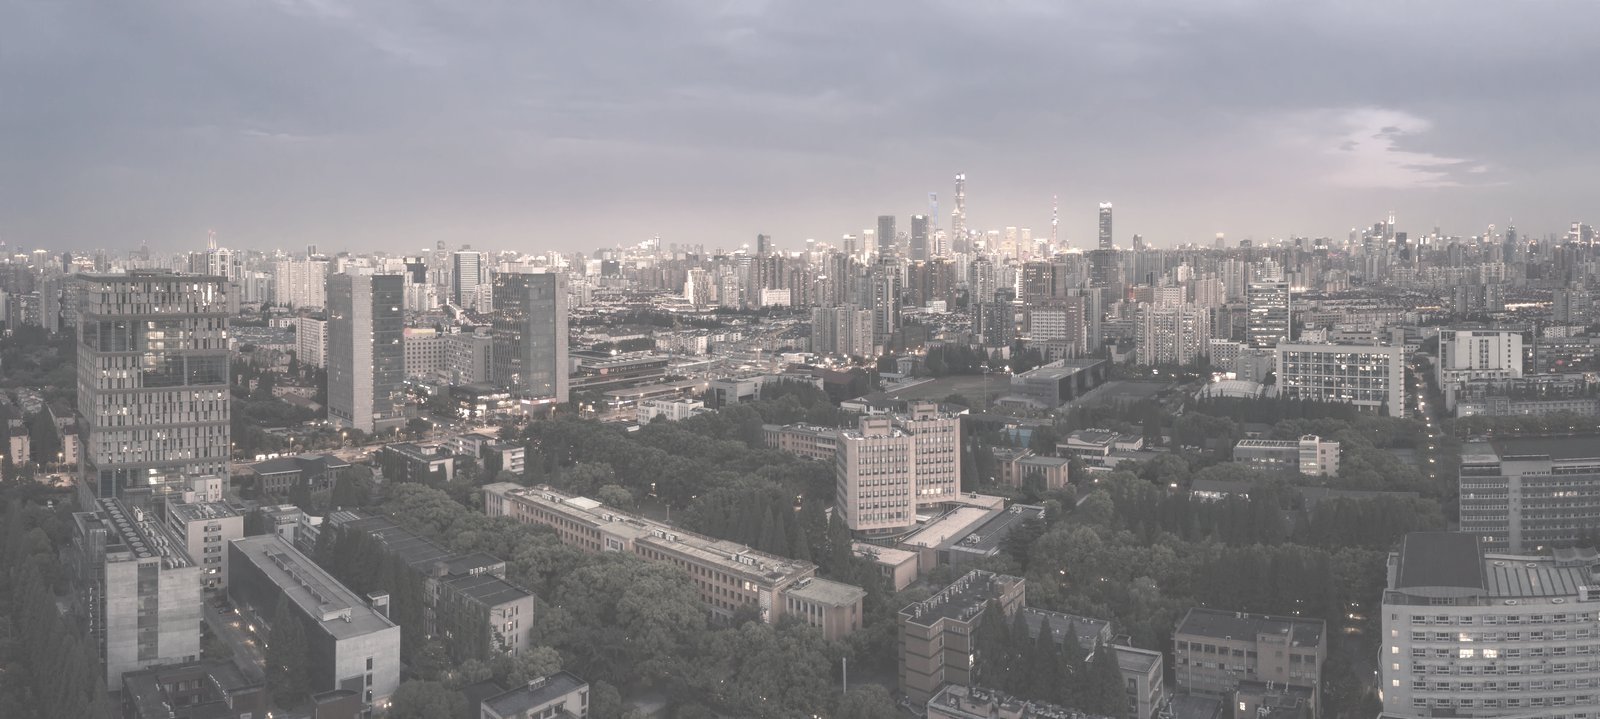
\includegraphics[width=\paperwidth,height=\paperheight,keepaspectratio=false]
        {tjvi/pics/03-cover.jpg}};

    % 白色蒙版（叠加在背景上、文字下）
    \fill[white, opacity=0.55]
      (current page.south west) rectangle (current page.north east);

    % 左上：小校徽
    \node[anchor=north west, inner sep=0pt]
      at ([xshift=0.06\paperwidth,yshift=-0.07\paperheight]current page.north west)
      {
\includegraphics[height=1.6cm]{tjvi/tongji-vi-badge.pdf}};

    % 中央偏左：主标题
    \node[anchor=west, text width=0.85\paperwidth, align=left, inner sep=0pt]
      at ([xshift=0.06\paperwidth,yshift=0.05\paperheight]current page.west)
      {{\sffamily\bfseries\color{cprimary}\fontsize{34pt}{40pt}\selectfont \TongjiBeamer{}}\\[0.6em]
       {\heiti\color{cprimary!85}\fontsize{18pt}{24pt}\selectfont 同济大学风格幻灯片模板}};

    % 底部：分隔线 + 信息行（取自 \author / \institute[短名] / \date）
    \draw[cprimary, line width=0.8pt]
      ([xshift=0.06\paperwidth,yshift=0.16\paperheight]current page.south west)
      -- ([xshift=0.5\paperwidth,yshift=0.16\paperheight]current page.south west);
    \node[anchor=south west, inner sep=0pt]
      at ([xshift=0.06\paperwidth,yshift=0.08\paperheight]current page.south west)
      {{\sffamily\color{black!80}\small
        \insertauthor \quad|\quad \insertshortinstitute \quad|\quad \insertdate}};
  \end{tikzpicture}%
\end{frame}
}

\section{快速开始}

\begin{frame}[fragile]{加载主题}
  在 \texttt{ctexbeamer} 文档类下加载主题：
\begin{lstlisting}
\documentclass[aspectratio=169]{ctexbeamer}
\usetheme[max,blue,light]{tjbeamer}
\end{lstlisting}
  可选参数：
  \begin{itemize}
    \item \textbf{封面样式}：\texttt{max} / \texttt{maxplus} / \texttt{min}
    \item \textbf{主色调}：\texttt{blue}（同济蓝）/ \texttt{red}（同济红+金）
    \item \textbf{明暗}：\texttt{light} / \texttt{dark}
    \item \textbf{徽标位置}：\texttt{topright} / \texttt{bottomright}
  \end{itemize}
\end{frame}

\begin{frame}[fragile]{编译方式}
  本模板使用 \XeLaTeX{} 编译：
\begin{lstlisting}
latexmk -xelatex main.tex
\end{lstlisting}
  推荐使用提供的 \texttt{Makefile}：
\begin{lstlisting}
make            # 编译
make clean      # 清理中间文件
make cleanall   # 清理所有产物
\end{lstlisting}
\end{frame}

\begin{frame}[fragile]{两种视觉模式}
  通过 \texttt{main.tex} 顶部的开关切换：
\begin{lstlisting}
\newif\iftjbgmode
% \tjbgmodetrue    % 注释 = 简洁版（默认）
\tjbgmodetrue      % 取消注释 = 背景版
\end{lstlisting}
  \begin{itemize}
    \item \textbf{简洁版}：白底 + 右侧半隐校徽淡水印，适合答辩、严肃汇报。
    \item \textbf{背景版}：按节轮换同济地标低饱和照片做背景，适合宣讲、海报式报告。
  \end{itemize}
\end{frame}

\begin{frame}[fragile]{字体与排版}
  本模板字体设计：
  \begin{itemize}
    \item \textbf{标题}/Frame Title/Section：\textsf{Noto Sans CJK SC}（黑体）
    \item \textbf{正文}/列表/Block Body：Noto Serif CJK SC（宋体）
    \item \texttt{代码}：Noto Sans Mono CJK SC
    \item 备用书法体：\kaiti 霞鹜文楷（\texttt{\textbackslash{}kaiti} 切换）
  \end{itemize}
  内部还注册了三个 CJK 家族开关：
\begin{lstlisting}
{\heiti  黑体示例}    % Noto Sans CJK SC
{\songti 宋体示例}    % Noto Serif CJK SC
{\kaiti  楷体示例}    % LXGW WenKai
\end{lstlisting}
\end{frame}

\section{特性演示}

\begin{frame}{文本格式}
  支持各类强调和文本格式：
  \begin{itemize}
    \item 普通文本 \quad |\quad The quick brown fox jumps over the lazy dog.
    \item \textbf{加粗文本 Bold}
    \item \textit{斜体文本 Italic}
    \item \alert{警示文本（同济红）}
    \item \emph{强调文本}
    \item \uline{下划线文本}
    \item \texttt{等宽字体 typewriter}
  \end{itemize}
\end{frame}

\begin{frame}{块（Blocks）样式}
  \begin{block}{标准块}
    内容区域。块标题底色为同济蓝，正文区底色为浅蓝灰。
  \end{block}
  \begin{alertblock}{警示块}
    用于强调重要信息。底色为同济红。
  \end{alertblock}
  \begin{exampleblock}{示例块}
    用于展示示例内容。
  \end{exampleblock}
\end{frame}

\begin{frame}{列表与项目符号}
  \begin{columns}[T]
    \column{0.5\textwidth}
    \textbf{无序列表}：
    \begin{itemize}
      \item 第一项
      \item 第二项
        \begin{itemize}
          \item 子项 A
          \item 子项 B
        \end{itemize}
      \item 第三项
    \end{itemize}
    \column{0.5\textwidth}
    \textbf{有序列表}：
    \begin{enumerate}
      \item 第一步 -- 准备阶段
      \item 第二步 -- 执行阶段
      \item 第三步 -- 验证阶段
    \end{enumerate}
  \end{columns}
\end{frame}

\begin{frame}{表格}
  \centering
  \begin{tabular}{lrr}
    \toprule
    项目 & 数值 A & 数值 B \\
    \midrule
    指标一 & 0.725 & 0.612 \\
    指标二 & 0.699 & 0.534 \\
    指标三 & 0.640 & 0.487 \\
    \midrule
    平均   & 0.688 & 0.544 \\
    \bottomrule
  \end{tabular}
  \vspace{1em}\\
  \footnotesize\color{ctertiary} 表 1：使用 \texttt{booktabs} 绘制的三线表
\end{frame}

\begin{frame}{数学公式}
  \begin{equation}
    \mathcal{L}(\theta) = -\sum_{i=1}^{N} \log p_\theta(y_i \mid x_i)
  \end{equation}
  行内公式：$E = mc^2$ 与 $\nabla \cdot \mathbf{E} = \rho/\varepsilon_0$。
  \begin{align}
    f(x) &= a_0 + \sum_{n=1}^{\infty} \left[ a_n \cos(nx) + b_n \sin(nx) \right] \\
    a_n  &= \frac{1}{\pi} \int_{-\pi}^{\pi} f(x) \cos(nx) \, dx
  \end{align}
\end{frame}

\begin{frame}{图片与图表}
  \begin{columns}[T,onlytextwidth]
    \column{0.48\textwidth}
    \centering
    
\includegraphics[height=3.6cm]{tjvi/tongji-vi-badge.pdf}\\[0.4em]
    {\footnotesize 图~1：嵌入矢量 PDF（校徽）}
    \column{0.48\textwidth}
    \centering
    \begin{tikzpicture}
      \draw[cprimary, line width=1pt] (0,0) -- (4,0) -- (4,2.4) -- (0,2.4) -- cycle;
      \draw[cprimary!50, dashed] (0,0) -- (4,2.4);
      \draw[cprimary!50, dashed] (4,0) -- (0,2.4);
      \node[cprimary] at (2,1.2) {\bfseries TikZ 绘制};
    \end{tikzpicture}\\[0.4em]
    {\footnotesize 图~2：TikZ 原生矢量图形}
  \end{columns}
\end{frame}

\begin{frame}[fragile]{代码高亮}
  \texttt{lstlisting} 已配置好同济蓝高亮风格：
\begin{lstlisting}
\documentclass[aspectratio=169]{ctexbeamer}
\usetheme[max,blue,light]{tjbeamer}

\title{Tongji-Beamer 答辩演示}
\author{您的姓名}
\date{\today}

\begin{document}
  \maketitle
  \section{引言}
  ...
\end{document}
\end{lstlisting}
\end{frame}

\begin{frame}{定理、定义、证明}
  \begin{theorem}[勾股定理]
    直角三角形两直角边平方和等于斜边平方：$a^2 + b^2 = c^2$。
  \end{theorem}
  \begin{definition}[凸集]
    集合 $C \subseteq \mathbb{R}^n$ 称为凸集，若 $\forall x, y \in C$ 与 $\lambda \in [0, 1]$，有 $\lambda x + (1-\lambda) y \in C$。
  \end{definition}
  \begin{proof}
    略。
  \end{proof}
\end{frame}

\begin{frame}{逐步显示（Overlay）}
  Beamer 的 \texttt{\textbackslash{}pause} 与 \texttt{<n->} 让内容按顺序出现：
  \begin{itemize}
    \item<1-> 第一步：先看到这一项
    \item<2-> 第二步：然后这一项浮现
    \item<3-> 第三步：最后才出现
  \end{itemize}
  \only<3->{\vspace{1em}\textit{用于答辩时引导观众注意力。}}
\end{frame}

\begin{frame}{多列布局与图标}
  \begin{columns}[T,onlytextwidth]
    \column{0.33\textwidth}
    \centering
    \faGithub\\[0.3em]\small 源码托管
    \column{0.33\textwidth}
    \centering
    \faFilePdf\\[0.3em]\small 矢量输出
    \column{0.33\textwidth}
    \centering
    \faPalette\\[0.3em]\small 统一视觉
  \end{columns}
  \vspace{0.8em}
  \begin{block}{`fontawesome5` 提供 1500+ 图标}
    用 \texttt{\textbackslash{}faGithub}、\texttt{\textbackslash{}faRocket}、\texttt{\textbackslash{}faLightbulb} 等命令直接嵌入图标。
  \end{block}
\end{frame}

\begin{frame}{链接与跳转}
  \begin{itemize}
    \item 外链：\href{https://github.com/sjtug/SJTUBeamer}{SJTUBeamer 项目主页}（点击跳转）
    \item URL：\url{https://github.com/TJ-CSCCG/tongji-visual}
    \item 邮箱：\href{mailto:example@tongji.edu.cn}{example@tongji.edu.cn}
    \item \faArrowRight~\hyperlink{frame_end}{跳转到致谢页}
  \end{itemize}
  \vspace{0.6em}
  \footnotesize\color{ctertiary}
  \texttt{\textbackslash{}hypertarget} + \texttt{\textbackslash{}hyperlink} 可实现幻灯片间跳转。
\end{frame}

\section{视觉素材}

\begin{frame}{同济视觉素材展示}
  \begin{columns}[c,onlytextwidth]
    \column{0.32\textwidth}
    \centering
    
\includegraphics[height=3cm]{tjvi/tongji-vi-badge.pdf}\\[0.5em]
    \footnotesize 同济校徽（蓝色版）
    \column{0.32\textwidth}
    \centering
    
\includegraphics[height=3cm]{tjvi/tongji-vi-vlogo.pdf}\\[0.5em]
    \footnotesize 同济校徽（紫色版）
    \column{0.32\textwidth}
    \centering
    
\includegraphics[width=0.9\linewidth]{tjvi/tongji-vi-zhlogo.pdf}\\[0.5em]
    \footnotesize 同济大学校名
  \end{columns}
  \vspace{1em}
  \footnotesize\color{ctertiary} 矢量素材均来自
  \href{https://github.com/TJ-CSCCG/tongji-visual}{TJ-CSCCG/tongji-visual}。
\end{frame}

\begin{frame}{颜色定义}
  \begin{columns}[c]
    \column{0.5\textwidth}
    \textbf{蓝色调（默认）}
    \vspace{0.5em}\\
    \tikz\fill[tjBluePrimary]   (0,0) rectangle (1,0.5); \texttt{tjBluePrimary}\\[0.3em]
    \tikz\fill[tjBlueSecondary] (0,0) rectangle (1,0.5); \texttt{tjBlueSecondary}\\[0.3em]
    \tikz\fill[tjBlueTertiary]  (0,0) rectangle (1,0.5); \texttt{tjBlueTertiary}\\
    \column{0.5\textwidth}
    \textbf{红色调（red 选项）}
    \vspace{0.5em}\\
    \tikz\fill[tjRedPrimary]   (0,0) rectangle (1,0.5); \texttt{tjRedPrimary}\\[0.3em]
    \tikz\fill[tjRedSecondary] (0,0) rectangle (1,0.5); \texttt{tjRedSecondary}\\[0.3em]
    \tikz\fill[tjRedTertiary]  (0,0) rectangle (1,0.5); \texttt{tjRedTertiary}\\
  \end{columns}
  \vspace{1.5em}
  \footnotesize 主题代码统一通过 \texttt{cprimary} / \texttt{csecondary} / \texttt{ctertiary} 抽象引用。
\end{frame}

\section{进阶用法}

\begin{frame}[fragile]{自定义封面}
  本模板封面在 \texttt{main.tex} 的 \texttt{自定义封面} 区块直接以 TikZ overlay 写就，
  完全可自由替换。常见自定义：
  \begin{itemize}
    \item 替换背景图：改 \texttt{tjvi/pics/03-cover.jpg}
    \item 调整白色蒙版透明度：\texttt{\textbackslash{}fill[white, opacity=0.55]}
    \item 修改标题字号 / 颜色 / 位置：直接编辑该区块中的 \texttt{\textbackslash{}node} 参数
  \end{itemize}
\end{frame}

\begin{frame}[fragile]{文件组织建议}
  对于稍长的演讲，可以按节拆分：
\begin{lstlisting}
% main.tex
\begin{document}
  \input{sections/cover.tex}
  \input{sections/01-intro.tex}
  \input{sections/02-method.tex}
  \input{sections/03-results.tex}
  \input{sections/thanks.tex}
\end{document}
\end{lstlisting}
  每个文件里只放 \texttt{\textbackslash{}section\{...\}} 和该节的 frames。
\end{frame}

\begin{frame}{背景按节轮换（背景版）}
  开启 \texttt{\textbackslash{}tjbgmodetrue} 后，每个 section 切换不同同济地标做大背景：
  \begin{itemize}
    \item §1 之前（致谢区）：蝴蝶桥航拍（\texttt{01-bg.jpg}）
    \item §1：仰望星空大楼（\texttt{02-bg.jpg}）
    \item §2：航拍同济（\texttt{03-bg.jpg}）
    \item §3：春雨中的校园（\texttt{04-bg.jpg}）
  \end{itemize}
  替换 \texttt{tjvi/pics/} 下的图片或在 \texttt{\textbackslash{}AtBeginSection} 中调整顺序即可换素材。
\end{frame}

% ====================================================================
% 致谢与来源（倒数第二页，保留页码与右侧水印 = 普通内容页）
% ====================================================================
\begin{frame}{致谢与来源}
  \hypertarget{frame_end}{}
  \begin{itemize}
    \item \textbf{原始模板}：\TongjiBeamer{} fork 自
      \href{https://github.com/sjtug/SJTUBeamer}{SJTUBeamer}
      （CC-BY-NC-SA 4.0）
    \item \textbf{视觉素材}：校徽与校名矢量图来自
      \href{https://github.com/TJ-CSCCG/tongji-visual}{TJ-CSCCG/tongji-visual}；\\
      内容页矢量水印组合及背景图思路参考
      \href{https://github.com/Kian-Chen/TongjiBeamer}{Kian-Chen/TongjiBeamer}。
    \item \textbf{颜色}：同济蓝 RGB(50, 90, 160)。
    \item \textbf{字体}：Noto Sans / Serif CJK SC + 霞鹜文楷 LXGW WenKai（均开源）。
    \item 本模板仅供同济大学相关学习、教学、答辩等非商业用途。
  \end{itemize}
\end{frame}

% ====================================================================
% 谢谢页 —— 仓库链接占位，使用前请替换 your-username/your-repo
% 同样禁用右侧水印
% ====================================================================
{
\tjbgenabledfalse
\setbeamertemplate{navigation symbols}{}  % 谢谢页隐藏页码与导航
\begin{frame}[plain,noframenumbering]
  \centering
  \vspace*{2cm}
  
\includegraphics[height=2.6cm]{tjvi/tongji-vi-badge.pdf}\par
  \vspace{1.2em}
  {\Huge\bfseries\color{cprimary} 谢\,谢}\par
  \vspace{1em}
  {\Large 欢迎反馈与贡献}\par
  \vspace{1.8em}
  {\footnotesize\color{black!70}
    \faGithub~\href{https://github.com/your-username/your-repo}{github.com/your-username/your-repo}}
\end{frame}
}

\end{document}
